\subsection{Grafo com Suporte à Anotação Semântica}\label{4-grasews-grafo}

O principal componente visual de Grasews é o grafo. Grasews utiliza a notação visual proposta no Capítulo \ref{3-notacao-visual-para-sawsdl} para representar hierarquicamente elementos de uma especificação WSDL e classes de uma ontologia OWL, possibilitando que um usuário crie anotações semânticas segundo a abordagem SAWSDL. Para os elementos WSDL/XSD passíveis de serem anotados com \textit{Model Reference}, Grasews disponibiliza um menu de contexto para adicionar e remover um URI de \textit{Model Reference}. Para os elementos passíveis de serem anotados tanto com \textit{Model Reference} quanto com \textit{Lifting Schema Mapping} e \textit{Lowering Schema Mapping}, Grasews estende o menu de contexto anterior com opções adicionais para permitir todos os tipos de anotações. A \figurename~\ref{fig:grasews-grafo-tipo-complexo-contexto} ilustra o menu de contexto disponível para um tipo complexo XSD \texttt{GetAllBooks} (parcialmente visível atrás do menu de contexto).

A \figurename~\ref{fig:grasews-grafo-model-reference} apresenta parte do grafo de uma especificação WSDL anotada com \textit{Model Reference}. Observa-se que a interface \texttt{MyWebSerice} está anotada com \textit{Model Reference} utilizando a classe OWL \texttt{ExpressionContent}, esta pertencente à ontologia \texttt{books}. Adicionalmente, a operação \texttt{MyMethodB} está anotada com \textit{Model Reference} utilizando a classe OWL \texttt{Article}, da mesma ontologia. Grasews constrói automaticamente a estrutura hierárquica entre as duas classes OWL em uso por anotações semânticas. Com isso, as classes OWL intermediárias \texttt{LinguisticExpression} e \texttt{Text} são automaticamente dispostas no grafo entre as duas classes OWL \texttt{ExpressionContent} e \texttt{Article}.

\begin{landscape}
    \begin{figure}[h]
        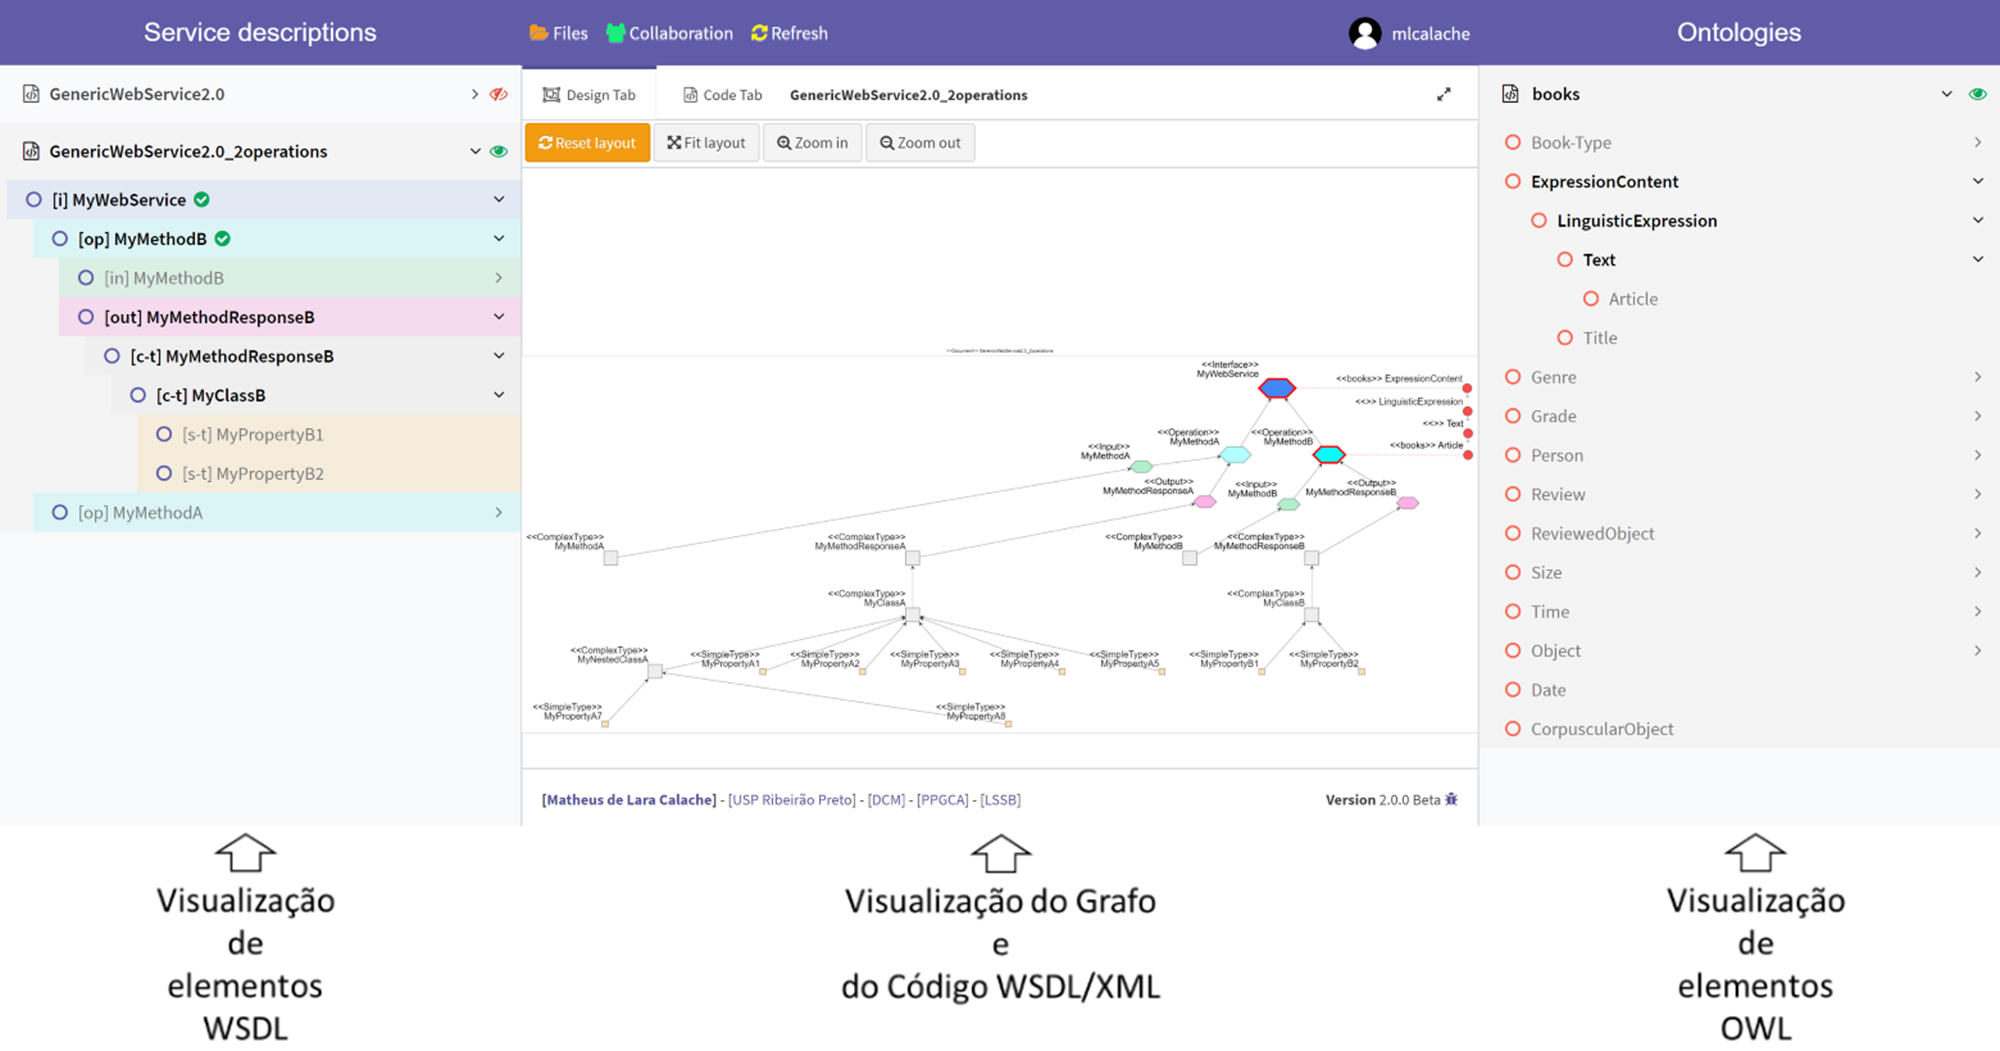
\includegraphics[scale=0.45]{4-grasews/imagens/grasews.png}
        \centering
        \caption[Interface gráfica de Grasews]{\textbf{Interface gráfica de Grasews.}}
        \label{fig:grasews}
    \end{figure}
\end{landscape}

Adicionalmente, Grasews provê um painel para visualizar o código XML de uma especificação WSDL. A \figurename~\ref{fig:grasews-painel-codigo} ilustra o painel de visualização do código WSDL/XML. O painel é automaticamente atualizado conforme o trabalho (anotações semânticas) é realizado. Com isso, caso o usuário tenha conhecimento técnico no código XML de uma especificação WSDL, este usuário pode verificar o painel de código a fim de validar as anotações semânticas criadas com o auxílio das notações visuais de Grasews. Entretanto, o painel de visualização de código não é editável.

\begin{figure}[h]
    %\resizebox{\textwidth}{!}{
        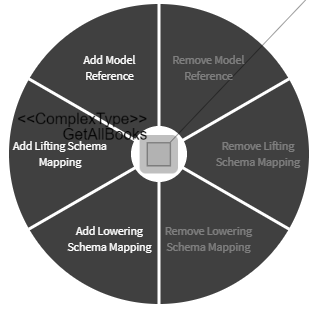
\includegraphics[scale=0.8]{4-grasews/imagens/grasews-grafo-tipo-complexo-contexto.png}
    %}
    \centering
    \caption[Menu de contexto para anotação semântica por meio do grafo de Grasews]{\textbf{Menu de contexto para anotação semântica por meio de grafo do Grasews.}}
    \label{fig:grasews-grafo-tipo-complexo-contexto}
\end{figure}

\begin{figure}[h]
    \resizebox{\textwidth}{!}{
        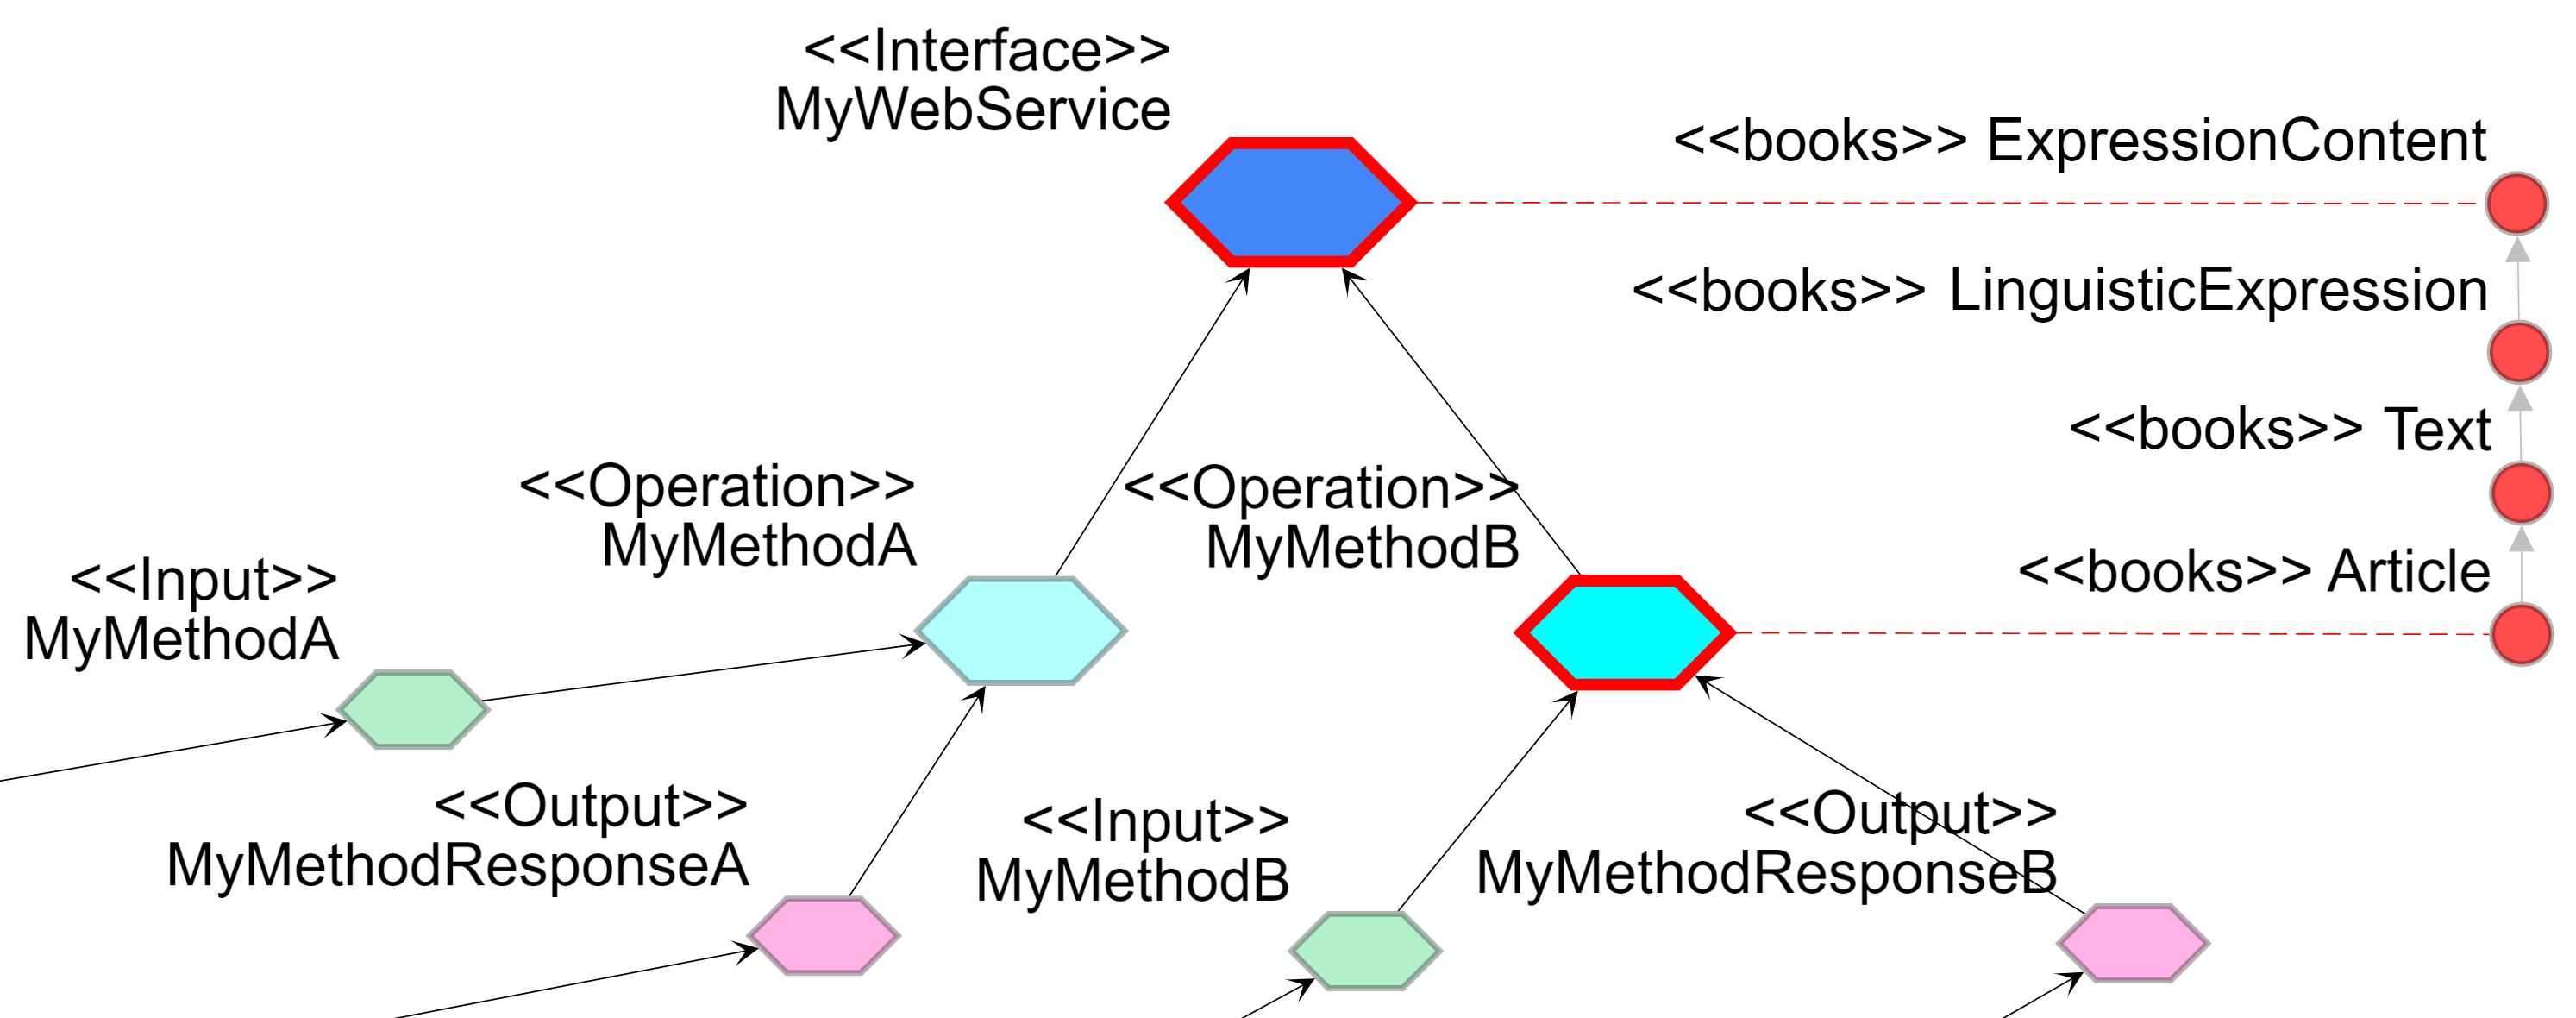
\includegraphics[scale=0.8]{4-grasews/imagens/grasews-grafo-model-reference.png}
    }
    \centering
    \caption[Elementos do grafo de Grasews anotados com \textit{Model Reference}]{\textbf{Elementos do grafo de Grasews anotados com \textit{Model Reference}.}}
    \label{fig:grasews-grafo-model-reference}
\end{figure}

\begin{figure}[h]
    \resizebox{\textwidth}{!}{
        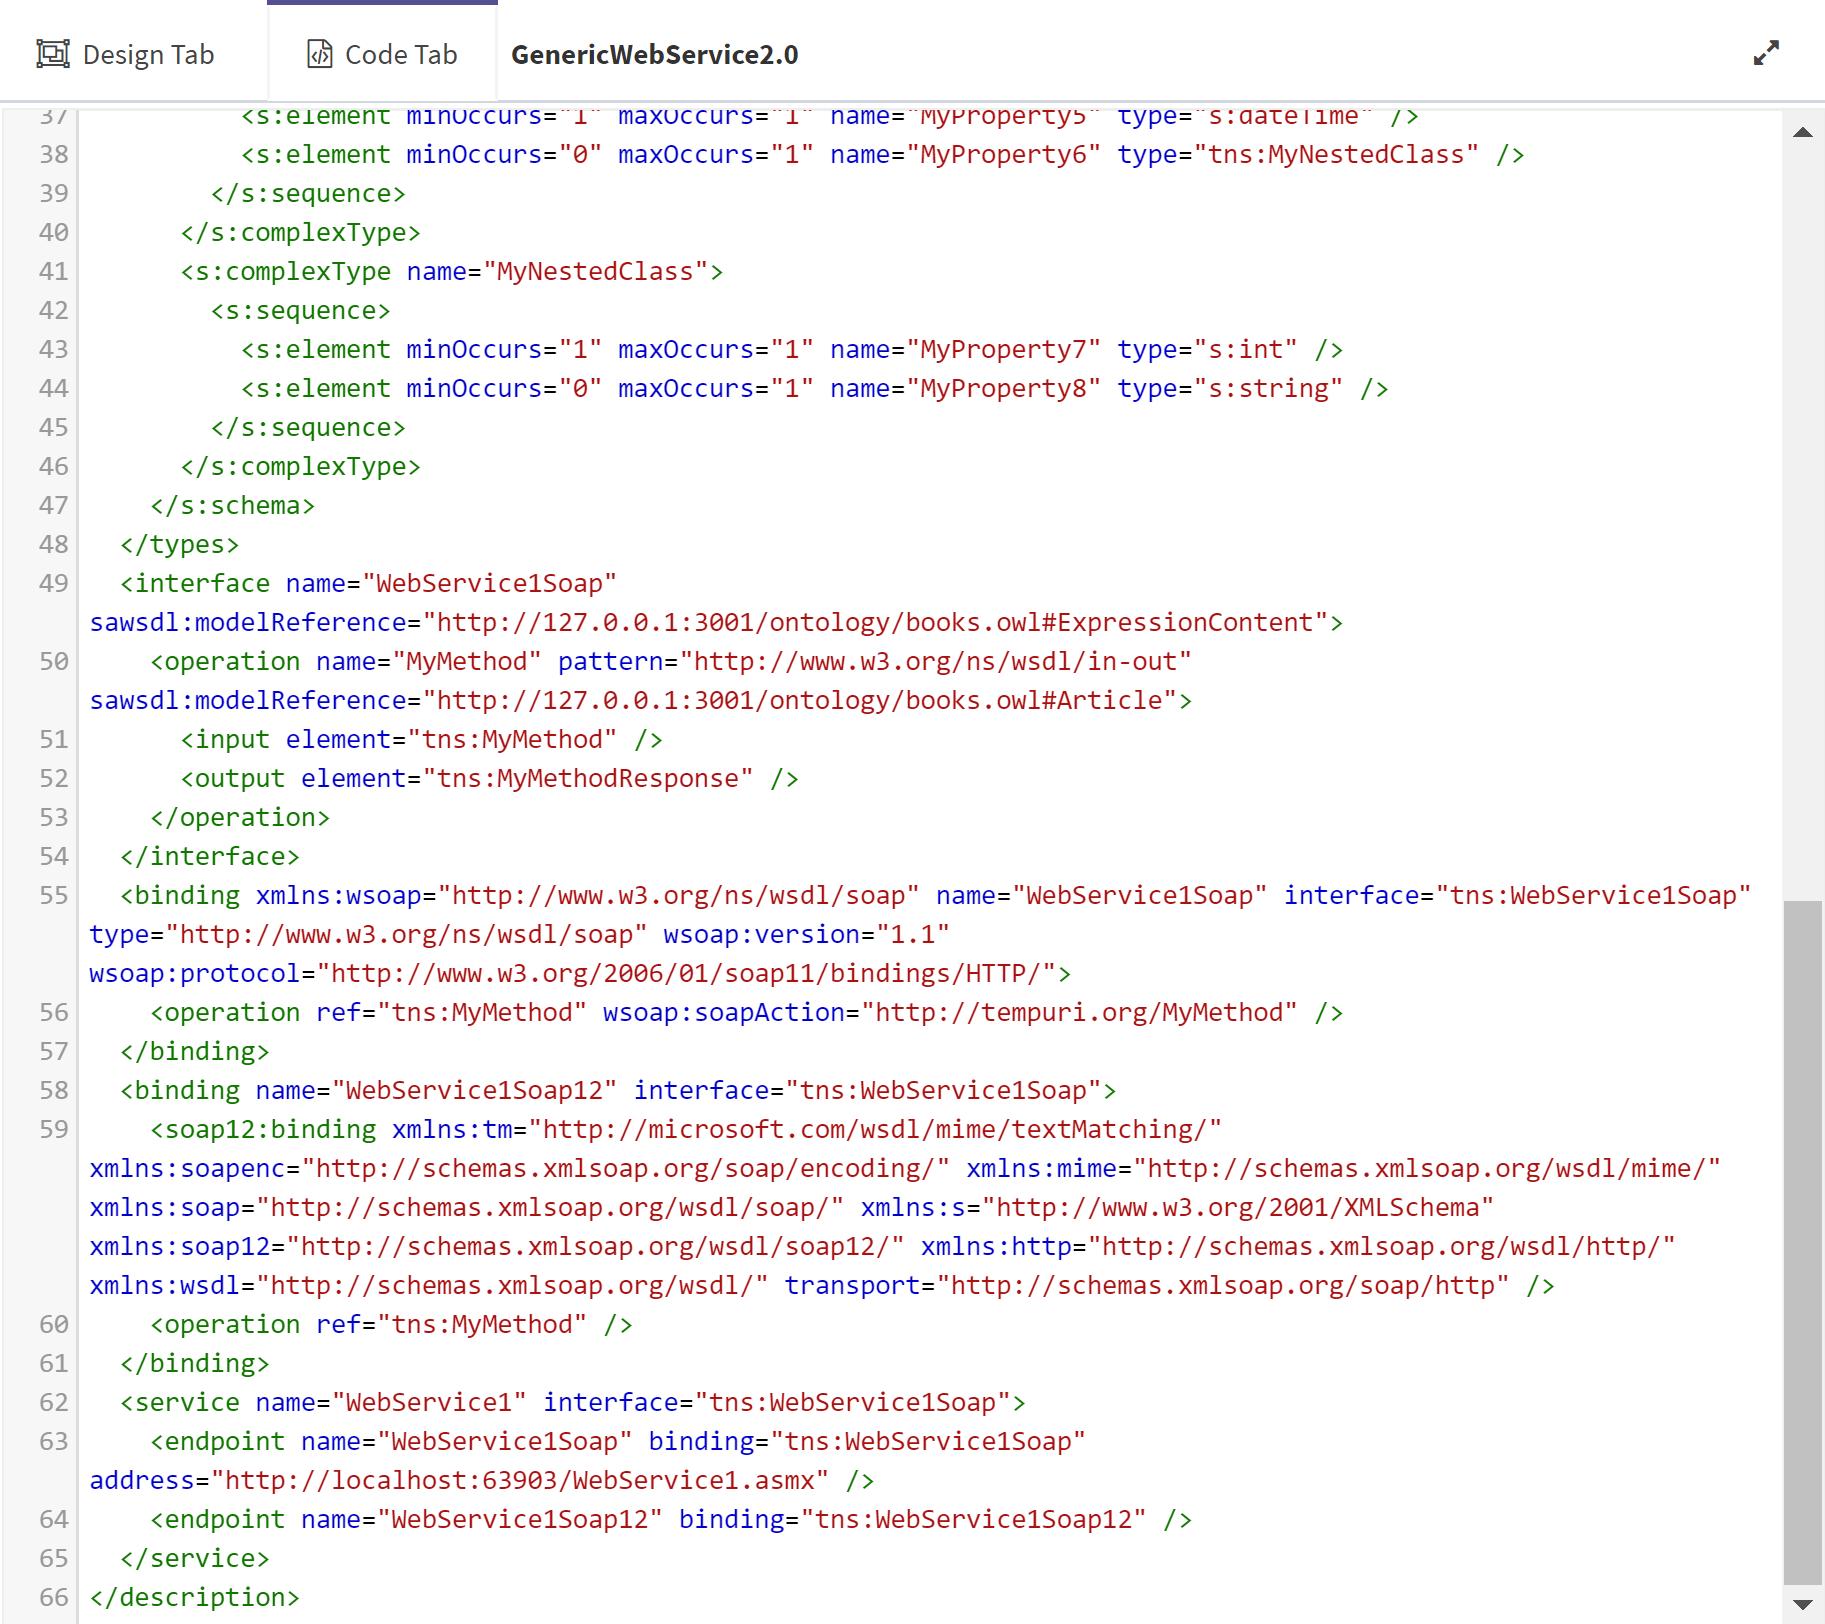
\includegraphics[scale=0.250]{4-grasews/imagens/grasews-painel-codigo.png}
    }
    \centering
    \caption[Painel de Grasews para visualização do código WSDL/XML]{\textbf{Painel de Grasews para visualização do código WSDL/XML.}}
    \label{fig:grasews-painel-codigo}
\end{figure}